
% \subsubsection{Naive Classifier}

% Four naive classification model are build according to this dataset, with $80\%$ training set and $20\%$ test set.

% \begin{table}[tbh!]
% \begin{tabular}{|l||l|l|} 
% \hline
% & Train error & Test error\\ 
% \hline
% \hline
% Logistic regression & 0.14990 & 0.15119\\
% \hline
% Random forest & 0.01998 & 0.13677\\
% \hline
% Linear discriminant analysis & 0.16213 & 0.16031\\
% \hline
% Support vector machine & 0.15488 & 0.15302\\
% \hline
% \end{tabular}
% \caption{Naive classification methods with standard settings: (1) assign positive for $p > 0.5$ in logistic regression; (2) ntree = 500 in random forest; (3) use maximum likelihood method in LDA; (4) use sigmoid kernel for SVM. }
% \label{tab:naive_model}
% \end{table}

% We compare the predictive performance of BQ with BART against the methods indicated in performance table (Table \ref{classification-performance}). Notably, the main Bayesian models that we wish to apply BQ with BART are the Gaussian process (GP) classification model with the logit link function $\sigma(p) = \log{[p/(1-p)]}$ as described in \cite{Rasmussen:2005:GPM:1162254}. Following a similar setup, given a training set $(X,y)$ and a test covariate $x_*$, we first approximate the posterior of the latent variable $f$, $p(f|X,y,x_*)$, by $q(f|X,y,x_*)$. This can be obtained either using the Laplace approximation or expectation propagation. Our predictive probability of class 1 is then 

% \begin{equation}
% p(y_* = 1|X,y,x_*) \approx \int_\mathbb{R} \sigma(f_*) q(f_*|X,y,x_*)df_*.
% \label{eq:predictprob}
% \end{equation}

% It is clear that if we had used the probit link function $\sigma(\cdot)=\Phi(\cdot)$ then (\ref{eq:predictprob}) would have a closed analytical form \cite{Rasmussen:2005:GPM:1162254}. 

% Since we do not know the exact form of the function $f$, it is not possible to compute this integral using BQ with GP, since the evaluation of the first term in (\ref{eqn:BQwithGP}) would not be attainable as we do not know the exact form of the function $f$. However, in the special where we are considering a Bayesian linear model (BLM), when $f(x) = x^Tw$, this is possible.

% Our procedure for BQ with BART is as follows. For each posterior draw $j$, we obtain $K$ functions $g_{\mbox{BART},j}^1,\ldots,g_{\mbox{BART},j}^K$ corresponding to the trees.

% \begin{table}
%     \caption{Performance of different models with respective inference methods on the classification of income bins on the "adults" dataset. The models involved are Gaussian process (GP), Bayesian linear models (BLM), support vector machines (SVM), random forest (RF) and XGBoost.}
%     \footnotesize
%     \begin{tabularx}{\columnwidth}{lcccc}
%     \hline
%     Model  & Method & Train. err.  & Test err.  \\
%     \hline
% GP (logit)      & Lapl. approx. + BART &  &  \\
%                 & Lapl. approx. + MI    &  &   \\
% GP (probit)     & Lapl. approx. &  &  \\
%                 &  Expec. prop. &  \\
% BLM             & Lapl. approx. + BART &  &  \\
%                 &  Expec. prop. + GP &  \\
% SVM             & MLE &  &     \\
% RF              & - &  &     \\
% XGBoost         & - &  &     \\
%     \hline
%     \end{tabularx}
%     \label{classification-performance}
% \end{table}

Our design is applicable to real-life problems, for example, surveying. 

Suppose we have a small set of census data with response and a list of information of potential candidates without response. Working with query design, we could avoid investigating response of every candidate but find the "best" ones to conduct the survey, hence decrease the cost of manual labour in the investigation. BART-BQ with sequential query design thus provides a good way to find the best candidates and then accurately compute the population metrics, such as mean income for our studies.

\subsection{Exploratory Data Analysis}

We obtained the 2017 ACS PUMS data on income in Wyoming \cite{ACS}, with attributes age, sex, race, education etc. We are going to predict the income of the observations. Figure~\ref{fig:income} shows the histogram of the distribution of income.

\begin{figure}[tbh!]
    \centering
    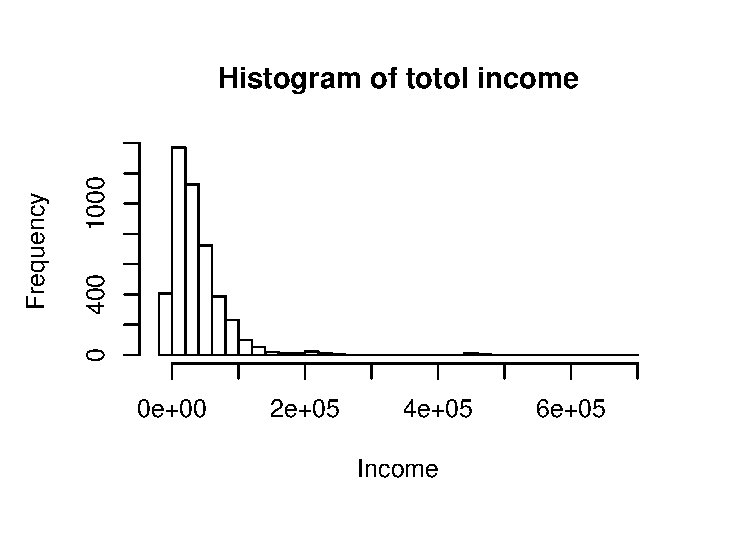
\includegraphics[width = 0.38\textwidth]{6.Real_Data_Sets/income.eps}
    \caption{Histogram of total income of an individual, normalised during training process.}
    \label{fig:income}
\end{figure}

We could further divide the data by sex (Figure~\ref{fig:by_sex}) to obtain finer data which is often required in real-life problems.

\begin{figure}[tbh!]
    \centering
    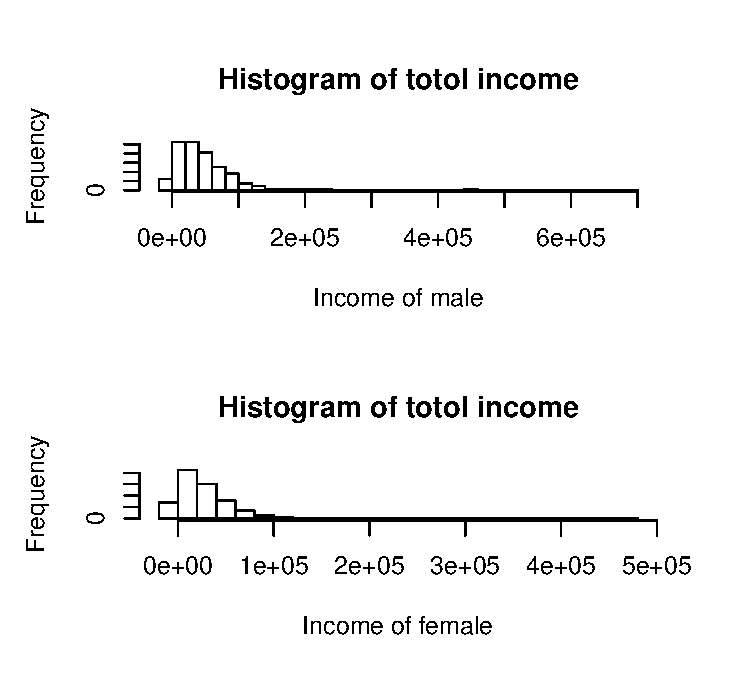
\includegraphics[width = 0.38\textwidth]{6.Real_Data_Sets/by_sex.eps}
    \caption{Histogram of total income by sex. The individual distributions have similar shape as in Figure~\ref{fig:income}, being normalised when training.}
    \label{fig:by_sex}
\end{figure}

\subsection{Experiment Design}
We are going to estimate the mean income of the whole population with a quarter of existing data and add $M$ "best candidates" to the survey by sequential design. We then stratify our data into male and female and then estimate the population mean for each category, using the same setup.

The reason for this is be understood in the setting where we are first given a database of existing census information $\mathcal{X}\times\mathcal{Y}$, where $\mathcal{X}$ are the population attributes and $\mathcal{Y}$ are the income, and we have the ability to send surveyors to $M$ individuals in a subset of size $n$ of the population. We already know the attributes of the $n$ individuals but we have to survey to obtain their income information. We then select exactly the best $M$ individuals to survey such that we can best estimate the population mean with BART-BQ, using the surveyed income information. Algorithm~\ref{alg:RLSQ} describes the precise design of the survey.
\begin{algorithm}[tbh!]
  \caption{Sequential Design for Survey}
  \label{alg:RLSQ}
\begin{algorithmic}
  \STATE {\bfseries Input:} \\existing census information $\mathcal{X}\times\mathcal{Y} = \{(x_i, y_i)\}_{i=1}^n$,  \\candidate set $\mathcal{C} = \{c_1, \ldots, c_L\}$ \\
  $M$ number of new samples to collect
  \FOR{$M$ iterations}
  \STATE fit BART of $K$ trees with $\mathcal{X}$ and $\mathcal{Y}$
  \STATE find $f_{\mbox{BART}}^{(1)}(c), \ldots, f_{\mbox{BART}}^{(K)}(c)$ for all $c\in\mathcal{C}$
  \STATE compute the empirical variance $\widehat{\mbox{Var}}[(f_{1}(c),..,f_{N}(c))]$
  \STATE Find $\,c^* = \mbox{argmax}_{c} \widehat{\mbox{Var}}[(f_{1}(c),..,f_{N}(c))]$
	\label{eq:maxvar}
  \STATE obtain the total income $y_c^*$ of the selected candidate
  \STATE $\mathcal{D} \leftarrow \mathcal{D}\cup \{c^*\}$, $\mathcal{C} \leftarrow \mathcal{C}\setminus \{c^*\}$
  \STATE $\mathcal{Y} \leftarrow \mathcal{Y}\cup \{y_c^*\}$
\ENDFOR
\end{algorithmic}
\end{algorithm}

BART-BQ method introduced in section~\ref{BQ-BART} will give us the estimation of expected income with increasing accuracy and decreasing variance. In the real world, the stopping criterion could be limited by budget of conducting the survey, labour, geographical limitation, etc.

Our existing competitors are simple random sample (Monte Carlo) and block random sampling. Block random sampling is a method of segmenting the data by specific attribute. For simplicity, we separate the data by sex. The principle is to sample the same ratio of male and female candidates from candidates and conduct the survey, to obtain sample mean and variance.

For this particular dataset, we use 25\% as training set and 25\% as the "approachable candidates". The remaining is left out of the survey design, as in real life they would be classified as not approachable.

\subsection{Experimental Results}



% \begin{table}[tbh!]
% \caption{Naive regression methods with standard settings: (1) ntree = 500 in random forest; (2) use maximum likelihood method in LDA; (3) use sigmoid kernel for SVM. (4) ntree = 50 in BART. The square root of MSE is printed.}
% \label{tab:naive_model}
% \vskip 0.15in
% \begin{center}
% \begin{small}
% \begin{sc}
% \begin{tabular}{lcccr}
% \toprule
% & Train MSE & Test MSE\\
% \midrule
% Linear regression & 0.0647 & 0.0636\\
% Random forest & 0.00911 & 0.02018\\
% LDA & 680.2146 & 658.8549\\
% SVM & 64.4301 & 63.4421\\
% %BART & 0.0239 & 0.0274\\
% \bottomrule
% \end{tabular}
% \end{sc}
% \end{small}
% \end{center}
% \vskip -0.1in
% \end{table}

% \subsection{Advanced Model Structure}

% In this section, we are going to perform \textcolor{red}{(how many?)} models with more advanced structure to obtain approximations of $E(y|x)$. 

% The comparison on MSE will be made among GP with BQ, BART with BQ, Monte Carlo method and \textcolor{red}{(other methods?)}.

% The advanced BART-BQ regression model modifies the method mentioned in BART \cite{BART}. 

% For a new data point $x$ and a BART model with functions $f^1_{j\mbox{BART}},\ldots,f^{ntree}_{j\mbox{BART}}$ in the $j$th posterior draw, each tree 

% \begin{table}[tbh!]
%     \caption{Performance of different models with respective inference regression methods on clustering coefficient on the network dataset. }
%     \footnotesize
%     \begin{tabularx}{\columnwidth}{lcccc}
%     \hline
%     Model  & Method & Train MSE & Test MSE  \\
%     \hline
% GP (logit)      & Lapl. approx. + BART &  &  \\
%                 & Lapl. approx. + MI    &  &   \\
% GP (probit)     & Lapl. approx. &  &  \\
%                 &  Expec. prop. &  \\
% BLM             & Lapl. approx. + BART &  &  \\
%                 &  Expec. prop. + GP &  \\
% SVM             & MLE &  &     \\
% RF              & - &  &     \\
% XGBoost         & - &  &     \\
%     \hline
%     \end{tabularx}
%     \label{classification-performance}
% \end{table}